%CONTEUDO DO ARQUIVO TESE.TEX, NOSSO ARQUIVO PRINCIPAL
\documentclass[fleqn, a4paper, 12pt]{report}
\setlength{\mathindent}{0pt}

\usepackage{latexsym}

\usepackage[utf8]{inputenc}
\usepackage{pslatex}
%\renewcommand{\familydefault}{\sfdefault}

\usepackage[T1]{fontenc}



\usepackage{geometry}
 \geometry{
 a4paper,
 top=3cm,
 bottom=3cm
 }



\usepackage{boxhandler}


\usepackage{float}
\usepackage{threeparttable}
\usepackage{caption}
\usepackage{subcaption}
\captionsetup{%
   labelsep=newline,
   justification=raggedright,
   labelfont=md,
   figurewithin=none,
  singlelinecheck=off
}
\usepackage[table,dvipsnames]{xcolor}
\usepackage{multicol}
\usepackage{tcolorbox}
\DeclareCaptionLabelSeparator{dash}{\;\texttwelveudash\;}
%\DeclareCaptionLabelFormat{nonumber}{}

\captionsetup{singlelinecheck = false,justification=centering, font=normalsize,textfont=bf, labelsep=dash,labelfont=bf}
\usepackage{newfloat}
\usepackage{titletoc}
\usepackage[titles]{tocloft}

\usepackage{tocbasic}


\DeclareFloatingEnvironment[
fileext=loq,
listname={Lista de Quadros},
within=none
]{quadro}

\newlistof{ilustr}{loil}{\hfill \bf LISTA DE ILUSTRAÇÕES\hfill}
\makeatletter
% Change the file extension of both lot and lof
\def\ext@quadro{loil}
% Store the original `\thefigure` and `\thetable`
\let\tohe@thequadro\thequadro
% Redefine them to contain a "dummy" `\tohe@list...`
\def\thequadro{\tohe@listquad\tohe@thequadro}
% Make the two dummy commands truly dummy
\let\tohe@listquad\relax
% Store the original `\listoffigtab`
\let\tohe@listofilustr\listofilustr
% Redefine it in such a way that the dummy commands insert "Fig." or "Tab." respectively
\def\listofilustr{%
  \begingroup
  \def\tohe@listquad{Quadro ~}
  \tohe@listofilustr
  \endgroup  
}
\makeatother

\newlistof{figs}{lofig}{\hfill \bf LISTA DE FIGURAS\hfill}
\makeatletter
% Change the file extension of both lot and lof
\def\ext@figure{lofig}
% Store the original `\thefigure` and `\thetable`
\let\tohe@thefigure\thefigure
% Redefine them to contain a "dummy" `\tohe@list...`
\def\thefigure{\tohe@listfig\tohe@thefigure}
% Make the two dummy commands truly dummy
\let\tohe@listfig\relax
% Store the original `\listoffigtab`
\let\tohe@listoffigs\listoffigs
% Redefine it in such a way that the dummy commands insert "Fig." or "Tab." respectively
\def\listoffigs{%
  \begingroup
  \def\tohe@listfig{Figura ~}
  \tohe@listoffigs
  \endgroup  
}
\makeatother

\DeclareFloatingEnvironment[
fileext=loc,
name=Código,
listname={Lista de Códigos},
within=none
]{codigo}


\newlistof{cods}{locods}{\hfill \bf LISTA DE CÓDIGOS\hfill}
\makeatletter
% Change the file extension of both lot and lof
\def\ext@codigo{locods}
% Store the original `\thefigure` and `\thetable`
\let\tohe@thecodigo\thecodigo
% Redefine them to contain a "dummy" `\tohe@list...`
\def\thecodigo{\tohe@listcod\tohe@thecodigo}
% Make the two dummy commands truly dummy
\let\tohe@listcod\relax
% Store the original `\listoffigtab`
\let\tohe@listofcods\listofcods
% Redefine it in such a way that the dummy commands insert "Fig." or "Tab." respectively
\def\listofcods{%
  \begingroup
  \def\tohe@listcod{Código ~}
  \tohe@listofcods
  \endgroup  
}
\makeatother




\newcommand*\MeasuredFigureLabel[1]{
    
}

\newcommand{\BFIG}[1]{ 
\captionsetup{singlelinecheck=off,labelfont=md,justification=raggedright}

\begin{figure}[H]\centering\begin{measuredfigure}\caption{\textmd{#1}}\hspace{-0.18cm}\centering\begin{tabular}{l}}
\newcommand{\EFIG}[2]{\\ {\footnotesize #1}\end{tabular}\end{measuredfigure}\addtocounter{figure}{-1}\phantomcaption\label{#2}\end{figure}}

\newcommand{\BQUAD}[1]{
\captionsetup{singlelinecheck=off,labelfont=md,justification=raggedright}
\begin{quadro}[H]\centering\begin{measuredfigure}\hspace{-0.18cm}\caption{\textmd{#1}}\centering\begin{tabular}{l}}
\newcommand{\EQUAD}[2]{\\ {\footnotesize #1}\end{tabular}\end{measuredfigure}\addtocounter{quadro}{-1}\phantomcaption\label{#2}\end{quadro}}

\newcommand{\BTAB}[1]{
\captionsetup{singlelinecheck=off,labelfont=md,justification=raggedright}
\begin{table}[H]\centering\begin{measuredfigure}\hspace{-0.18cm}\caption{\textmd{#1}}\centering\begin{tabular}{l}}
\newcommand{\ETAB}[2]{\\{\footnotesize#1}\end{tabular}\end{measuredfigure}\addtocounter{table}{-1}\phantomcaption\label{#2}\end{table}}

\newcommand{\BCOD}[1]{
\begin{center}
\begin{minipage}{0.78\textwidth}
\captionsetup{singlelinecheck=off,labelfont=md,justification=raggedright}
\begin{codigo}[H]\caption{\textmd{#1}}\tiny}
\newcommand{\ECOD}[2]{\label{#2}\vspace{3pt}{\footnotesize#1}\end{codigo}\end{minipage}\end{center}}

%Meus comandos


\usepackage{tgpagella}
%
\usepackage{amsmath}
\usepackage{amssymb}
\usepackage[amsmath]{ntheorem}
\usepackage[backgroundcolor=yellow!50,portuguese]{todonotes}
\newcommand{\tdl}[1]{\todo[inline]{\tiny #1}}
\usepackage[cache=false,newfloat]{minted}
\usepackage{pgf}
\usepackage{tikz}
\usetikzlibrary{calc,matrix,arrows,automata}
\usepackage{wrapfig}
\usepackage[final]{pdfpages}
\usepackage[pdftex, hidelinks]{hyperref}

\usepackage[portuguese,linesnumbered]{algorithm2e}
\usepackage{placeins}
%\usepackage{showlabels}
\usepackage{units}
\usepackage[alf]{abntex2cite}
%\usepackage[style=abnt,backend=biber]{biblatex}



\renewcommand\bibname{Reference}

\usepackage{pdfpages}
\usepackage{setspace}


\usepackage{fancyhdr}
\pagestyle{fancy}
\fancypagestyle{plain}{
    \fancyhf{} % clear all header and footer fields
    \fancyhead[RO,RE]{\thepage} %RO=right odd, RE=right even
    \renewcommand{\headrulewidth}{0pt}
    \renewcommand{\footrulewidth}{0pt}
}
\pagestyle{plain}
\usepackage{parskip}
\parskip=0.5pt

\newcommand{\argmin}[1]{\underset{#1}{\operatornamewithlimits{argmin}}\;}
\newcommand{\mini}[1]{\underset{#1}{\operatornamewithlimits{min}}\;}

\newcolumntype{R}{>{\columncolor{red!20}}r}
\newcolumntype{G}{>{\columncolor{green!20}}r}
\newcolumntype{B}{>{\columncolor{blue!20}}r}
\newcolumntype{Y}{>{\columncolor{yellow!20}}r}
\newcolumntype{K}{>{\columncolor{gray!20}}r}

\SetKwInput{Recebe}{Recebe}
\SetKwInput{Acao}{Ação}
\SetKwInput{Viz}{Vizibilidade}
\SetKwBlock{Inicio}{início}{fim}
\SetKw{Novo}{novo}
\SetKw{Deste}{deste}
\SetKw{Ou}{or}
\SetKw{Como}{como}
\SetKw{Ate}{até}
\SetKw{AlgE}{e}
\SetKw{AlgOu}{ou}
\SetKw{AlgNao}{não}
\SetKw{Falso}{falso}
\SetKw{Thread}{thread}
\SetKw{Verdadeiro}{verdadeiro}
\SetKwFunction{PL}{Problema\_Linear}
\SetKwFunction{TL}{Tamanho\_da\_Lista}
\SetKwFor{ParaCada}{para cada}{faça}{fim}
\SetKwFor{Enquanto}{enquanto}{faça}{fim}
\SetKwFor{Para}{para}{faça}{fim}
\SetKwSwitch{Selecione}{Caso}{Outros}{selecione}{faça}{caso}{outros}{fim da seleção}

\newcommand{\argmax}{\operatornamewithlimits{argmax}}

\newcommand{\CM}[1]{\CommentSty{\# #1 \#}}
\newcommand{\ins}[2]{#1 \longleftarrow #1 \cup \lbrace #2 \rbrace}

\definecolor{light-gray}{gray}{0.8}


\usepackage{latexsym}
\usepackage{theorem}
\usepackage{times}
\usepackage{amscd}
%\usepackage{epsf}
\usepackage{graphicx}
\usepackage{cancel}
\usepackage[all]{xy}
\usepackage{enumerate}
\usepackage{wrapfig}
\usepackage{indentfirst}
%\usepackage{setspace}
\usepackage{varioref}
\usepackage{color}
\usepackage{lscape}
\usepackage{longtable}
\usepackage[normalem]{ulem}
%\usepackage{tabularx}
%% \usepackage[light,timestamp]{draftcopy}
%% \draftcopySetGrey{0.9}
%% \usepackage[rflt]{floatflt}
%\usepackage[a4paper]{geometry}
\usepackage{ulem}
\usepackage{array}
\usepackage{multirow}
\usepackage{textcomp}
% %\usepackage{makeidx}
% %\usepackage{algorithm}
% \usepackage{algorithmic}
% %\makeindex
% %\renewcommand{\thetable}{\arabic{chapter}\Roman{table}}
\usepackage{csquotes}
\usepackage[brazilian]{babel}

\newcommand{\CC}{\mathbb{C}}
\newcommand{\EE}{\mathbb{E}}
\newcommand{\FF}{\mathbb{F}}
\newcommand{\NN}{\mathbb{N}}
\newcommand{\PP}{\mathbb{P}}
\newcommand{\QQ}{\mathbb{Q}}
\newcommand{\RR}{\mathbb{R}}
\newcommand{\ZZ}{\mathbb{Z}}
\newcommand{\RP}{\mathbb{RP}}

\newcommand{\mS}{\mathcal{S}}
\newcommand{\mU}{\mathcal{U}}
\newcommand{\mF}{\mathcal{F}}
\newcommand{\mG}{\mathcal{G}}
\newcommand{\mP}{\mathcal{P}}
\newcommand{\mQ}{\mathcal{Q}}
\newcommand{\mR}{\mathcal{R}}

\newcommand{\MS}{\mathscr{S}}
\newcommand{\MU}{\mathscr{U}}
\newcommand{\MF}{\mathscr{F}}
\newcommand{\MG}{\mathscr{G}}
\newcommand{\MP}{\mathscr{P}}
\newcommand{\MQ}{\mathscr{Q}}
\newcommand{\MR}{\mathscr{R}}

\newcommand{\norm}[1]{{\| #1 \|}}
\newcommand{\abs}[1]{{\vert #1 \vert}}

\newcommand{\setaright}{\longrightarrow}
\newcommand{\setaleft}{\longleftarrow}
\newcommand{\se}{\Longleftarrow}
\newcommand{\sose}{\Longrightarrow}
\newcommand{\sesose}{\Longleftrightarrow}
\newcommand{\setafunc}{\longrightarrow}
\newcommand{\f}[2]{f:#1\longrightarrow #2}
\newcommand{\fAB}{\f{A}{B}}
\newcommand{\fXY}{\f{X}{Y}}
\newcommand{\func}[3]{#1:#2\longrightarrow #3}
\newcommand{\F}{\longrightarrow}

\newcommand{\dv}[2]{\frac{\partial #1}{\partial #2}}
\newcommand{\dvu}[3]{\frac{\partial^2 #1}{\partial #2 \partial #3}}
\newcommand{\dvv}[2]{\frac{\partial^2 #1}{\partial #2^2}}
\newcommand{\raio}{\sqrt{1 + f_x^2 + f_y^2 + f_z^2}}
\newcommand{\ud}{\frac{1}{2}}
\newcommand{\uq}{\frac{1}{4}}

\newcommand{\Frac}[2]{\frac{\displaystyle #1}{\displaystyle #2}}
\newcommand{\Frace}[2]{\Frac{\ #1\ }{\ #2\ }}

\newcommand{\uu}[1]{\underline{#1}}

\newcommand{\Dx}{\Delta x}
\newcommand{\Dy}{\Delta y}
\newcommand{\Dz}{\Delta z}
\newcommand{\Posto}{\textrm{Posto}}
\newcommand{\Hess}{\textrm{Hess}}
\newcommand{\Det}{\textrm{Det}}

\newcommand{\bct}{\begin{center}}
\newcommand{\ect}{\end{center}}
\newcommand{\bsld}{\begin{slide}}
\newcommand{\esld}{\end{slide}}

\newcommand{\sen}{\operatorname{sen}}
\newcommand{\wt}{\widetilde}
\newcommand{\pp}{\,}
\newcommand{\CG}{Computação Gráfica}
\newcommand{\Rdo}{$^{\underline{\textrm{o}}}$ }
\newcommand{\Rda}{$^{\underline{\textrm{a}}}$ }

\newcommand{\Ac}{\{\,} %% Abre conjunto
\newcommand{\Fc}{\,\}} %% Fecha conjunto
\newcommand{\Conj}[1]{\Ac #1 \Fc}

\newtheorem{exemplo}{Exemplo}[chapter]
\newtheorem{exercicio}{Exercício}[chapter]
 \newtheorem{teorema}{Teorema}[chapter]
 \newtheorem{definicao}{Definição}[chapter]
 \newtheorem{observacao}{Observação}[chapter]
 \newtheorem{problema}{Problema}[chapter]
 \newtheorem{corolario}{Corolário}[chapter]
 \newtheorem{proposicao}{Proposição}[chapter]
 \newtheorem{lema}{Lema}[chapter]
 \newcommand{\dsp}{\displaystyle}
 \renewcommand{\thefootnote}{\alph{footnote}}


\newcommand{\OBS}{\textbf{Observação: }}
\newcommand{\lr}{L^2(\mathbb{R})}
\newcommand{\Demo}{\textit{Demonstração: }}
\newcommand{\fDemo}{$\Box$}

\newcommand{\His}{\hspace*{\parindent}} %% Horizontal indent space
\newcommand{\uHis}{\hspace*{1\parindent}}
\newcommand{\dHis}{\hspace*{2\parindent}}
\newcommand{\tHis}{\hspace*{3\parindent}}
\newcommand{\qHis}{\hspace*{4\parindent}}
\newcommand{\cHis}{\hspace*{5\parindent}}
\newcommand{\fatPar}{0.5}
\newcommand{\fatParEq}{0.7}

\newcommand{\bb}{\begin{equation}}
\newcommand{\ee}{\end{equation}}
\makeatletter
\@fleqnfalse
\@mathmargin\@centering
\makeatother

\newcounter{Letra}
\newcounter{letraTmp}
\newcommand{\letraZero}{\setcounter{Letra}{0}}
\newcommand{\Letra}[1]{\setcounter{Letra}{#1}}
\newcommand{\letraTmp}[1]{\setcounter{letraTmp}{#1}}

\newcommand{\boxEqSize}{6cm}
\newcommand{\boxSize}[1]{\renewcommand{\boxEqSize}{#1}}

\newcommand{\boxEqMat}[3]{\makebox[#1][l]{(#2) $#3$}}

\newcommand{\itMatLet}[1]{
\renewcommand{\theLetra}{\stepcounter{Letra}\alph{Letra}}
\boxEqMat{\boxEqSize}{\theLetra}{#1}}

\newcommand{\itMatNum}[1]{
\renewcommand{\theLetra}{\stepcounter{Letra}\arabic{Letra}}
\boxEqMat{\boxEqSize}{\theLetra}{#1}}


\newcommand{\boxEqPot}[3]{\makebox[#1][l]{(#2) #3}}

\newcommand{\itPotLet}[1]{
\renewcommand{\theLetra}{\stepcounter{Letra}\alph{Letra}}
\boxEqPot{\boxEqSize}{\theLetra}{#1}}

\newcommand{\itPotNum}[1]{
\renewcommand{\theLetra}{\stepcounter{Letra}\arabic{Letra}}
\boxEqPot{\boxEqSize}{\theLetra}{#1}}


\newcommand{\itLet}[1]{%% indexacao por letra
\renewcommand{\theLetra}{\stepcounter{Letra}\alph{Letra}}
(\theLetra) #1}

\newcommand{\itNum}[1]{%% indexacao por numero
\renewcommand{\theLetra}{\stepcounter{Letra}\arabic{Letra}}
\theLetra ) #1}

\newcommand{\boxEqMatSn}[2]{\makebox[#1][l]{$#2$}}
\newcommand{\Mat}[1]{\boxEqMatSn{\boxEqSize}{#1}}

\newcommand{\boxEqPotSn}[2]{\makebox[#1][l]{#2}}
\newcommand{\Pot}[1]{\boxEqPotSn{\boxEqSize}{#1}}


\newcommand{\Nm}[1]{\textnormal{#1}}
\newcommand{\Nume}{\operatorname{n}}
\newcommand{\Num}[1]{\Nume (#1)}

\newcounter{numQuestao}
\newenvironment{questoes}{
\begin{list}
{\arabic{numQuestao}- }
{\usecounter{numQuestao}\setlength{\labelwidth}{0.6cm}\setlength{\labelsep}{0cm}%
\setlength{\leftmargin}{0.6cm}}}
{\end{list}}


\newcommand{\tamBox}[1]
{
\boxSize{#1}
\letraZero
}
\newcommand{\itemBox}[1]{\item\tamBox{#1}}
\newcommand{\itemZero}{\letraZero\item}

\newcommand{\Tq}{\,|\,}

\newcommand{\newLet}{\letraTmp{\value{Letra}}\letraZero}
\newcommand{\oldLet}{\Letra{\value{letraTmp}}}
\newcommand{\comp}{\Nm{\footnotesize{$\circ$}}}

\newcommand{\fmu}{f^{-1}}

\usepackage{listings}



\cftsetindents{chapter}{0em}{8em}
\cftsetindents{section}{0em}{8em}
\cftsetindents{subsection}{0em}{8Em}

\addto\captionsbrazilian{
  \renewcommand{\contentsname}%
  {\hfill\textbf{\normalsize SUMÁRIO}\hfill}%
}
\addto\captionsbrazilian{
  \renewcommand{\listfigurename}%
  {\hfill\textbf{\normalsize LISTA DE FIGURAS}\hfill}%
}
\addto\captionsbrazilian{
  \renewcommand{\listtablename}%
  {\hfill\textbf{\normalsize LISTA DE TABELAS}\hfill}%
}
\addto\captionsbrazilian{
  \renewcommand{\bibname}%
  {\hfill\textbf{\normalsize REFERÊNCIAS}\hfill}%
}
\renewcommand{\cftchapfont}{\normalsize\bfseries}
\renewcommand{\cftsecfont}{\footnotesize\bfseries}
\renewcommand{\cftsubsecfont}{\footnotesize\itshape\bfseries}

\renewcommand{\cftchappagefont}{\normalsize\bfseries}
\renewcommand{\cftsecpagefont}{\normalsize\bfseries}
\renewcommand{\cftdot}{$\cdot$}
\renewcommand{\cftfigfont}{\normalsize}
\renewcommand{\cfttabfont}{\normalsize}

\renewcommand{\cftchapleader}{\cftdotfill{\cftdotsep}} 
\renewcommand{\cftsecleader}{\cftdotfill{\cftdotsep}} 

\usepackage{titlesec}

\titleformat{\chapter}[block]
{\normalsize\bfseries}
{\normalsize\bfseries\thechapter}
{12pt}
{}
\titleformat{\section}[block]
{\normalsize\bfseries}
{\normalsize\bfseries\thesection}
{12pt}
{}
\titleformat{\subsection}[block]
{\normalsize\bfseries\itshape}
{\normalsize\bfseries\itshape\thesubsection}
{12pt}
{}



\usepackage{chngcntr}  

%\counterwithout{figure}{chapter}
\counterwithout{table}{chapter}
\counterwithout{listing}{chapter}

\setlength\cftbeforefigskip{10pt}
\setlength\cftbeforetabskip{10pt}

\renewcommand{\cftfigpresnum}{}
\renewcommand{\cftfigaftersnum}{\hfill \texttwelveudash\;\;}

\renewcommand{\cfttabpresnum}{Tabela \ }
\newlength{\mylenf}
\settowidth{\mylenf}{\cftfigpresnum}
\setlength{\cftfignumwidth}{\dimexpr\mylenf+6.5em}
\setlength{\cfttabnumwidth}{\dimexpr\mylenf+6.5em}



\newenvironment{citacao}% environment name
{%
  \vspace{0.5cm}%
\begin{flushright}%
    \singlespacing
    \footnotesize%
    \begin{minipage}{10cm}
}{%
    \end{minipage}%
\end{flushright}\vspace{0.5cm}%
}% end code


\newlength{\bibitemsep}\setlength{\bibitemsep}{.2\baselineskip plus .05\baselineskip minus .05\baselineskip}
\newlength{\bibparskip}\setlength{\bibparskip}{0.5cm}
\let\oldthebibliography\thebibliography
\renewcommand\thebibliography[1]{%
  \oldthebibliography{#1}%
  \setlength{\parskip}{\bibitemsep}%
  \setlength{\itemsep}{\bibparskip}%
}
\newcommand{\req}[1]{(\ref{#1})}

\makeatletter
\def\memph{\@memph}
\def\@memph#1{%
  \protect\leavevmode
  \begingroup
    \color{red}{\mathbf{#1}}%
  \endgroup
}
\makeatother




% %\listfiles
 \onehalfspacing %é pra ser o comando do espaçamento 1.5
 \setlength{\parindent}{1.5cm}
 \setlength{\hoffset}{-0.5cm}
 \setlength{\voffset}{-1cm}
 \setlength{\textwidth}{16cm}
 \setlength{\textheight}{23.5cm}
 

\begin{document}

\onehalfspacing
 \newgeometry{
 a4paper,
 top=3cm,
 bottom=1cm
 }
\pagenumbering{gobble}

\begin{titlepage}
  \begin{figure}[htb]			
	  \centering
	  
\includegraphics[width=0.15\textwidth]{figuras/ifce.png}
  \end{figure}
  \begin{center}
    \textbf{INSTITUTO FEDERAL DE EDUCAÇÃO, CIÊNCIA E TECNOLOGIA DO CEARÁ}\\
    \textbf{IFCE \textit{CAMPUS} CEDRO}\\
    \textbf{LICENCIATURA EM MATEMÁTICA}\\

  \end{center}

 
\centering
	\begin{center}
	
		\vfill
		\textbf{NOME COMPLETO \\} 
\vfill
		\textbf{TÍTULO DO TRABALHO}\\
		
		
		
		
	\end{center}
	 \vfill
		
			\textbf{CEDRO - CE \\ 2021}
\end{titlepage}

\begin{titlepage}

\begin{center}
\textbf{ALBERT RAYNEER QUEIROZ DE QUEIROZ\\}
\vspace{7,5cm}

		\textbf{ARQUITETURA ESCALÁVEL PARA DESENVOLVIMENTO DE JOGOS DE QUIZ VOLTADO PARA EDUCAÇÃO INFANTIL EM PLATAFORMAS APPLE}\\

\vspace{2.5cm}

\vspace{2cm}
\begin{flushright}
	\begin{minipage}[l]{8cm}
		Trabalho de Conclusão de Curso apresentado ao Curso de Ciência da Computação do Instituto Federal de Educação, Ciência e Tecnologia do Ceará -IFCE - {\it{Campus}} Maracanaú como requisito para obtenção do Título de Bacharel em Ciência da Computação.\\
		Orientador: Prof. Me. Carlos Henrique Leitão Cavalcante.
	\end{minipage}
\end{flushright}

\end{center}

\vfill
\centering
		
			\textbf{Fortaleza - CE \\2021}

\end{titlepage}


%Esta é a ficha catalográfica, Não sei como você e seu orientador optaram para colocá-la, a minha está como imagem, se for fazer o mesmo retire os porcentos. 

%\newpage
%	\begin{figure}[b]		
%\vspace{12.0cm}

		%\includegraphics[scale=0.70]{figures/fichaficha}
	%\end{figure}

%\includepdf[pages={1}]{fichacatalografica.pdf} %fornecida pela biblioteca
%\includepdf[pages={1}]{folhadeaprovacao.pdf} %gerado pelo tex folhaaprovacao.tex assinado e escaneado

\begin{titlepage}
    \begin{center}
		
		\vspace{0.5cm}		
		NOME COMPLETO
		\vspace{0.5cm}
	\end{center}

		
	\begin{center}		
		\vspace{1cm}
		{\large {TÍTULO DO TRABALHO\\}}
		
		\vspace{3cm}
	\end{center}
	
	\begin{flushright}
	\begin{minipage}[l]{8cm}
	Esta Monografia foi julgada adequada para obtenção do título de Licenciado em matemática e aprovada em sua forma final pelo departamento de Matemática do Instituto Federal do Ceará-\textit{Campus} Cedro.
	
		\end{minipage}
\end{flushright}
			\vspace{3cm}

	Aprovado em: \rule{1.5cm}{0.1mm} / \rule{1.5cm}{0.1mm} / \rule{1.5cm}{0.1mm}
	
	\vspace{1.5cm}
	\begin{center}
	 	BANCA EXAMINADORA
	\end{center}
		
	\vspace{0.7cm}
	\begin{center}
		
		\rule{11cm}{0.1mm}
		
		Prof. Me. Luiz Fernando Ramos Lemos (Orientador)\\
		IFSULDEMINAS - \textit{Campus} Inconfidentes.
		
		
		\vspace{0.8cm}
		
		\rule{11cm}{0.1mm}
		
		Prof.(a). Ma. Mikaelle Barboza Cardoso\\
		IFCE - \textit{Campus} Sobral
		
		
		\vspace{0.8cm}
		\rule{11cm}{0.1mm}
		
		Prof. Dr. João Nunes de Araújo Neto\\
		IFCE - \textit{Campus} Cedro

		\vspace{3cm}
		

		

		
	\end{center}
	 \vfill
	 \centering
		
			%{\large Cedro - Ceará}
\end{titlepage}



\thispagestyle{plain}

\chapter*{}
\vspace{-4cm}
\begin{center}
 \textbf{DEDICATÓRIA}
\end{center}


\begin{center}

\begin{minipage}[c]{8cm}
\vspace{10cm}

À minha mãe, ...
\end{minipage}
\end{center}

\thispagestyle{plain}

\begin{flushright}
	\begin{minipage}[r]{6cm}
		\vspace{20cm}

		``Astronarta libertado\\
          Minha vida me urtrapassa\\
          Em quarqué rota que eu faça.''\\
		
		(Dois mil e um - Tom Zé)
		 
	\end{minipage}
\end{flushright}

\chapter*{}
\vspace{-4cm}
\begin{center}
 \textbf{AGRADECIMENTOS}
\end{center}

\vspace{0.5cm}
Graças à vida, que me deu tanto...

Ao Instituto Federal de Educação, Ciência e Tecnólogia do Ceará - \textit{Campus} Cedro, todos os servidores, professores e alunos.

Não esqueça de agradecer às instituições que lhe forneceram algum tipo de financiamento ao longo da graduação!!!




\chapter*{}
\vspace{-4cm}
\begin{center}
 \textbf{RESUMO}
\end{center}
\vspace{0.5cm}
\noindent
Resumo em português

\vspace{1cm}

\noindent {\bfseries Palavras-chave}: Desenvolvimento Mobile. Aplicativo. Whitelabel. Quiz. Arquitetura de Software. Educação. 


\chapter*{}
\vspace{-4cm}
\begin{center}
 \textbf{ABSTRACT}
\end{center}
\vspace{0.5cm}
\noindent
English abstract.
\vspace{1cm}

\noindent {\bfseries Keywords}: Mobile Development. Application. Whitelabel. Quiz. Software Architecture. Education.




\listofilustr
\listoffigs
\listofcods
\newpage
\renewcommand{\listtablename}{\hfill \bf LISTA DE TABELAS\hfill}
%\listoftables
\newpage
%\renewcommand
\tableofcontents

 \newgeometry{
 a4paper,
 top=3cm,
 bottom=3cm
 }

 \pagenumbering{arabic}
% \clearpage
\setcounter{page}{12}
  \chapter{INTRODUÇÃO}
\thispagestyle{empty}

Devido ao avanço do ensino a distância, cresceu a necessidade de criar ferramentas e recursos que fossem capazes de atrair a atenção dos alunos, principalmente os de idade menos elevada. Dado a evolução tecnológica e o contato cada vez mais frequente de crianças e jovens com aparelhos digitais, é inevitável anular a possibilidade de utilizar essas ferramentas como objetos de ensino. Visto isso, são inumeras as possibilidades para se aproveitar desses equipamentos.

Neste âmbito, foram realizadas diversas pesquisas relacionadas a eficácia da chamada "gamificação" no processo de aprendizagem, um exemplo de gamificação de questionários são os jogos de Quiz, que tem se tornado bastante populares e permitem abordar diferentes tipo de tema de forma lúdica e descontraída, como é mostrado por Carneiro (2014) em "Learning objects as enablers in distance education"\nocite{carneiro2014learning}, Vargas (2017) em "O processo de aprendizagem e avaliação através de
quiz"\nocite{vargas2017processo} e Bastos (2020) em "Quiz como ferramenta motivacional e avaliativa no ensino-aprendizagem de química."\nocite{bastos2020quiz}

Pensando nisso, alunos do IFCE, Campus Canindé, pesquisaram e desenvolveram um jogo quiz voltado para educação financeira de crianças na região rural, denominado Grana (2018)\nocite{pereira2018grana}. Após o desenvolvimento do projeto foram realizados estudos focados em analisar a sua eficácia no auxilio do ensino de gestão financeira, como é apresentado por Azevedo (2019)\nocite{azevedo2019analise} e Ramos (2020)\nocite{ramos2020analise}.

Além disso, o conceito de "white-label" tem ganhado popularidade no desenvolvimento de software, como explica Cann (2010). Cann define "white-labeling" como um produto ou serviço feito por uma compania e usado ou vendido por outras companias, esses produtos servem como base para um "rebrand" aonde é adicionada a identidade visual e marca da compania. Explica também que esse processo de "rebrand" pode ser realizado tanto pela empresa que produz quanto a que utiliza o "white-label".

Pensando nisso, esse trabalho busca aplicar o conceito de "white-label" para aplicações gamificadas no formato de quiz com o intuito de facilitar e/ou viabilizar o ensino de determinados temas ou assuntos para o público infantil. Para tal, será implementado um jogo quiz componentizado, seguindo os padrões de arquitetura limpa, com conteúdo personalizável, para plataformas Apple. Como exemplo de produto final, será utilizada a identidade visual e conteúdo do sistema previamente citado Grana (2018).
  \chapter{MOTIVAÇÃO INICIAL E JUSTIFICATIVA FUNDAMENTADA DO ESTUDO}
\label{cap1}
\thispagestyle{empty}

Apresente o que motivou o estudo e a justificativa da relevância e necessidade do estudo. O Quadro \ref{tabela-livro} é uma exemplo de quadro.

\BQUAD{LIVROS ANALISADOS}
  \begin{tabular}{|p{3cm}||c||p{4cm}|}
      \hline
      \textbf{Referência para citar no texto}    & \textbf {Título do livro} & \textbf {Autor/Autores} \\
  \hline
  \hline
  \label{livro 1}Livro 1 & Matemática Completa&Bonjorno, Giovanni Jr e Paulo Câmara \\ 
  \hline
 \label{livro 2}Livro 2 & Matemática: Contexto e Aplicações & Luiz Roberto Dante\\ 
 \hline
 \label{livro 3}Livro 3 & Matemática & Emanuel Paiva \\ 
 \hline
  \label{livro 4}Livro 4 & Matemática: Ciência e Aplicações  &Gelson Iezzi, Osvaldo Dulce, David Degenszajn, Roberto Périgo e Nilse de Almeida \\ 
  \hline
  \label{livro 5}Livro 5 & Matemática para compreender o mundo & Kátia Stocco Smole e Maria Ignez Diniz \\ 
 
 \hline
  \label{livro 6}Livro 6 & Fundamentos de Matemática Elementar & Gelson Iezzi e Carlos Marukami \\ 
 \hline

 \end{tabular}
\EQUAD{Fonte: Elaborado pela autor(a).}{tabela-livro}
\vspace{0.5cm}

 
  %INICIO DE CAPITULO
\chapter{FUNDAMENTAÇÃO TEÓRICA}
\label{cap:2}
\thispagestyle{empty}

Apresente um resumo das teorias utilizadas de forma a facilitar o acesso ao leitor do trabalho aos pré-requisitos para o entendimento do trabalho.

\section{Teoria dos Registros das Representações Semióticas}
\label{3.1}

 Ensinar é uma tarefa ...
O psicólogo e filósofo Raymond Duval, desenvolveu a Teoria dos Registros de Representação Semiótica - (TRRS)... 

A \emph{conversão} para \citeonline{colombo2008} é (exemplo de citação):

\begin{citacao}
 [...] a conversão de uma representação se refere às operações em que o registro inicial é transformado em outro registro; por essa razão, é considerada como uma “transformação externa”. Por exemplo, ao utilizarmos a linguagem algébrica para representar a frase “o dobro de um número resulta em oito”, estamos realizando uma conversão do registro dado na língua natural para o registro dado na linguagem algébrica \cite[p. 6]{colombo2008}.
\end{citacao}

Exemplo de figura.

\BFIG{Representação gráfica da função afim}

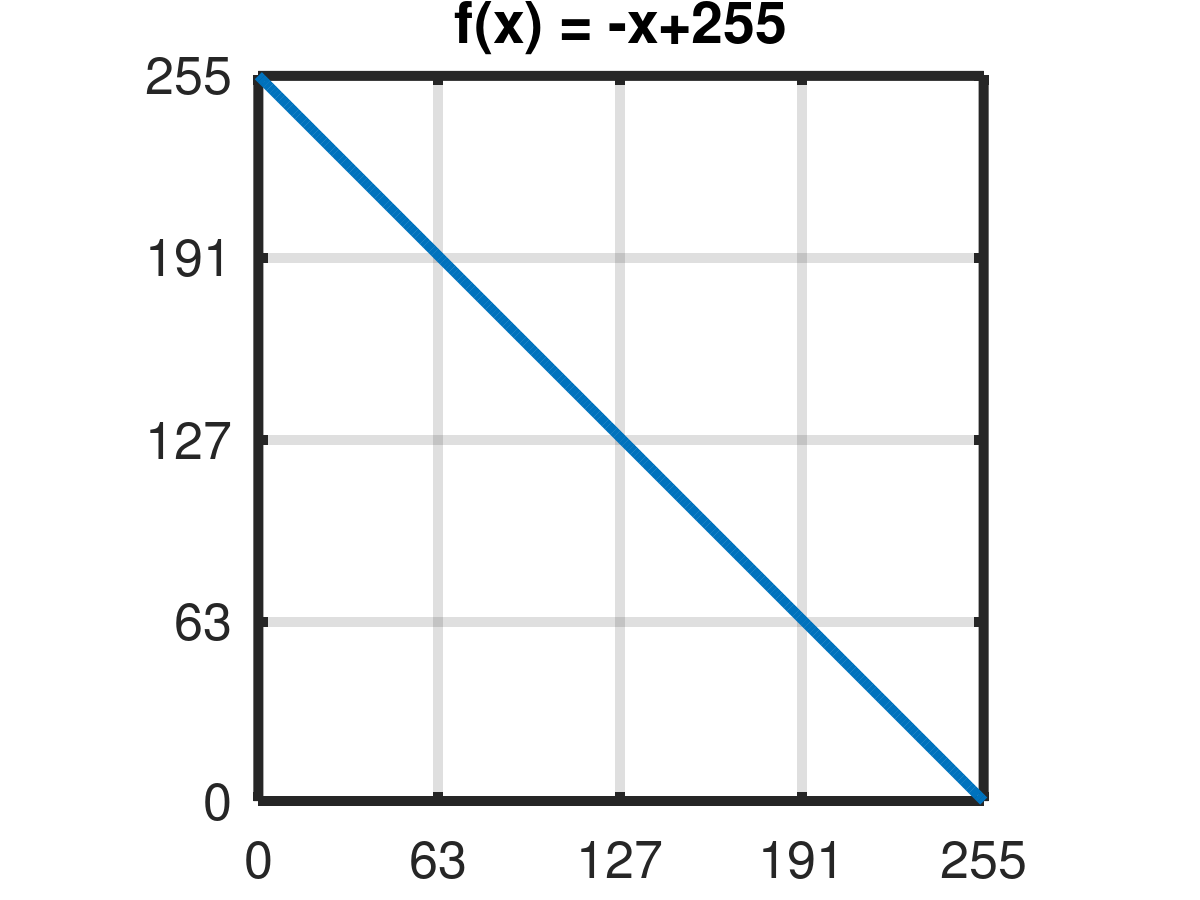
\includegraphics[width=0.60\linewidth]{./figuras/funcao.png}

\EFIG{Fonte: Elaborada pelo autor }{fig:repre}

Assim, a Figura \ref{fig:repre}..
	


\section{Exemplo de seção.}
\label{sec:introfunc}

\citeonline[p. 81]{murakami2004iezzi}, define Função como: 

\begin{definicao} 
Dado dois conjuntos $A$ e $B$, não vazios, uma relação $f$ de $A$ em $B$ recebe o nome de aplicação de $A$ em $B$ ou função definida em $A$ com imagens em $B$ se, e somente se, para todo $x\in A$ existe um só $y\in B$ tal que $(x,y)\in f$.

\bb
f\hspace{0.2cm} é\hspace{0.2cm} aplicado\hspace{0.2cm} de\hspace{0.2cm} A\hspace{0.2cm} em\hspace{0.2cm} B\hspace{0.2cm} \Longleftrightarrow (\forall \hspace{0.2cm} x \in A,\hspace{0.2cm} \exists \hspace{0.2cm} |y \in B|\hspace{0.2cm} (x,y)\in f) 
\ee

\end{definicao}


\subsection{Exemplo de subseção}
 \citeonline[p. 100] {murakami2004iezzi}, define função afim como:
 
 \begin{definicao}
 
  Uma aplicação de $\RR$ em $\RR$ com $a\neq 0$ e cada $x\in \RR$ associa o elemento $(a\cdot x + b)\in \RR$.

\bb
f(x)=a\cdot x+b\hspace{0.5cm} com \hspace{0.5cm}  (a\neq 0)
\ee

\end{definicao}
 
\subsection{Imagem da função afim}

\citeonline[p. 105] {murakami2004iezzi} diz que:

reta permitindo a análise de que todos os valores de $y$ estão relacionados com $x$. 

\subsection{Zero da função}


Vejamos que $f(x)$ é crescente pois na medida que os valores em $x$ vão aumentando, as suas respectivas imagens também crescem.\vspace{0.5cm}

\subsection{Exemplo de subseção}

\citeonline[p. 118]{murakami2004iezzi}, resume em:

 \begin{tcolorbox}[colback = white]
  A função afim: \bb\hspace{0.1cm} f(x)=a\cdot x+b\hspace{0.1cm}  anula-se\hspace{0.1cm} para\hspace{0.1cm} x= -\frac{b}{a}.\ee
  
  Para $x>-\frac{b}{a}$, temos:
\bb
\left \{ \begin{array}{rcl}
se\;  a>0\; \text{\textit{então}} \; f(x)=a\cdot x+b>0\\
se\; a<0\; \text{\textit{então}} \; f(x)=a\cdot x+b<0\\
\end{array}
\right.
\ee
Isto é, $x>-\frac{b}{a}$ a função $f(x)=a\cdot x+b$ tem sinal de a.\vspace{0.5cm}

Para $x<-\frac{b}{a}$, temos:
\bb
\left \{ \begin{array}{rcl}
se\;  a>0\; \text{\textit{então}} \; f(x)=a\cdot x+b<0 \\
se\; a<0\; \text{\textit{então}} \; f(x)=a\cdot x+b>0\\
\end{array}
\right.
\ee

Isto é, para $x<-\frac{b}{a}$ a função $f(x)=a\cdot x+b$ tem o sinal de ‘-a' (sinal contrário ao de a ).
\end{tcolorbox}

Exemplo de função definida por partes:
\begin{exemplo} 
Seja $f: \mathbb{R}\rightarrow \mathbb{R}$ definida por:

\bb
f(x) = \left \{ \begin{array}{rcl}
x & se & 0\leq x\leq 128\\
128 & se & 128\leq x\leq 256\\
x-128 & se &  c.c
\end{array}
\right.
\ee
\end{exemplo}

\section{Outra seção}
\label{sec:cod}

Exemplo de código.
\BCOD{Método da Bisseção}
 \begin{minted}[fontsize=\scriptsize]{matlab}
function xm=mb(f,xp,xn) % metodo da bissecao para zero de funcoes
  xm=(xp+xn)/2;
  y=f(xm);
  while(abs(y)>0.01) % enquanto |y|>ep -> laco de repeticao 
    if(y>0) % se y maior que 0
      xp=xm;
    else % senao
      xn=xm;
    end
    xm=(xp+xn)/2;
    y=f(xm);
  end
end
\end{minted}
\ECOD{Fonte: Elaborada pela autor(a) (GNU Octave)}{cod:mb} 
  \chapter{ABORDAGEM AO PROBLEMA}
 \label{cap3}
 \thispagestyle{empty}

Apresente a sua proposta de abordagem ao problema ou discussão da questão do trabalho monográfico.



 
 % \chapter{Outro capítulo}
\thispagestyle{empty}
\label{cap:outro}

 % Ativar caso queira o cap 4
  \chapter{CONSIDERAÇÕES FINAIS}
\thispagestyle{empty}
\markright{Considerações Finais}

Apresente suas considerações finais.

  \appendix 
  \renewcommand{\thechapter}{ANEXO A}

  \chapter{Apêndice}
\label{Ap}
\thispagestyle{empty}
\label{apendA}
\newpage

\section{Texto auxiliar do trabalho}

O apêndice deve ser autoral, textos externos devem ser colocados como anexo. 
  \renewcommand{\thechapter}{APÊNDICE B}
 % \chapter{APÊNDICE B: EXTRAS}
\thispagestyle{empty}
\label{apendB}
\newpage
 
  \renewcommand{\thechapter}{APÊNDICE C}
 % \include{ApendixC} 
  %\printindex 
  %\include{refer}
%  \printbibliography
  %\include{refs}  
  \bibliography{refs}
  \addcontentsline{toc}{chapter}{REFERÊNCIAS}

\end{document}  
